\subsection{Grammatical approach}

%#############################################################################################################%
%#############################################################################################################%
\iffalse
\begin{frame}[fragile]
  \frametitle{Example}

\begin{center}
  \alert{Where does the prime minister of United Kingdom live?}
\end{center}

\end{frame}
\fi
%#############################################################################################################%
%#############################################################################################################%

\begin{frame}[fragile]
  \frametitle{Dependency tree output by the Stanford Parser}

\begin{figure}
 \begin{tikzpicture}
  \node (0) at (10,10) {ROOT};
  \node (1) at (10,8.5) {live};
  \node (2) at (8,7) {minister};
  \node (3) at (10,7) {does};
  \node (4) at (12,7) {Where};
  \node (5) at (6,5.5) {the};
  \node (6) at (8,5.5) {prime};
  \node (7) at (10,5.5) {Kingdom};
  \node (8) at (10,4) {United};

  \node (9) at (14,1) {}; % utilisé pour forcer le positionnement de la figure globale

  \draw[->, >=latex] (0) edge node[anchor=center, right] {\scriptsize{root}} (1);
  \draw[->, >=latex] (1) edge node[anchor=center, left] {\scriptsize{nsubj}} (2);
  \draw[->, >=latex] (1) edge node[anchor=center, right] {\scriptsize{aux}} (3);
  \draw[->, >=latex] (1) edge node[anchor=center, right] {\scriptsize{advmod}} (4);
  \draw[->, >=latex] (2) edge node[anchor=center, left] {\scriptsize{det}} (5);
  \draw[->, >=latex] (2) edge node[anchor=center, right] {\scriptsize{prep\_of}} (7);
  \draw[->, >=latex] (2) edge node[anchor=center, left] {\scriptsize{amod}} (6);
  \draw[->, >=latex] (7) edge node[anchor=center, right] {\scriptsize{nn}} (8);
 \end{tikzpicture}
\end{figure}

\end{frame}

%#############################################################################################################%
%#############################################################################################################%

\begin{frame}[fragile]
  \frametitle{Preprocessing operation: merging}

\begin{figure}
 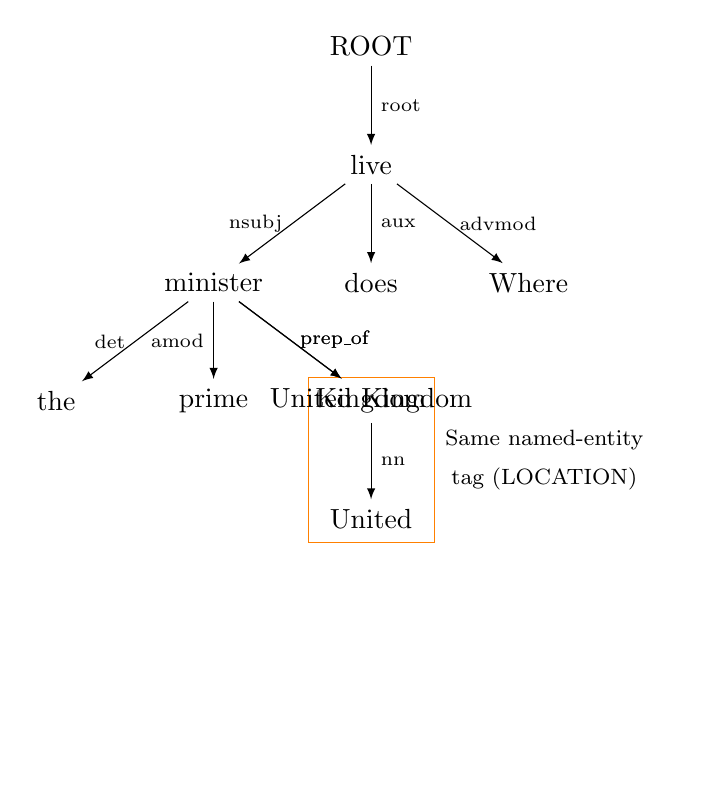
\begin{tikzpicture}
  \node (0) at (10,10) {ROOT};
  \node (1) at (10,8.5) {live};
  \node (2) at (8,7) {minister};
  \node (3) at (10,7) {does};
  \node (4) at (12,7) {Where};
  \node (5) at (6,5.5) {the};
  \node (6) at (8,5.5) {prime};
  \onslide<1>{\node (7) at (10,5.5) {Kingdom};}
  \onslide<1>{\node (8) at (10,4) {United};}

  \node (9) at (14,1) {}; % utilisé pour forcer le positionnement de la figure globale

  \onslide<1>{\draw [draw=orange] (9.2,5.8) rectangle (10.8,3.7);}
  \onslide<1>{\node (10) at (12.2,5) {\footnotesize{Same named-entity}};}
  \onslide<1>{\node (11) at (12.2,4.5) {\footnotesize{tag (LOCATION)}};}

  \onslide<2->{\node (12) at (10,5.5) {United Kingdom};}

  \draw[->, >=latex] (0) edge node[anchor=center, right] {\scriptsize{root}} (1);
  \draw[->, >=latex] (1) edge node[anchor=center, left] {\scriptsize{nsubj}} (2);
  \draw[->, >=latex] (1) edge node[anchor=center, right] {\scriptsize{aux}} (3);
  \draw[->, >=latex] (1) edge node[anchor=center, right] {\scriptsize{advmod}} (4);
  \draw[->, >=latex] (2) edge node[anchor=center, left] {\scriptsize{det}} (5);
  \onslide<1>{\draw[->, >=latex] (2) edge node[anchor=center, right] {\scriptsize{prep\_of}} (7);}
  \draw[->, >=latex] (2) edge node[anchor=center, left] {\scriptsize{amod}} (6);
  \onslide<1>{\draw[->, >=latex] (7) edge node[anchor=center, right] {\scriptsize{nn}} (8);}
  
  \onslide<2->{\draw[->, >=latex] (2) edge node[anchor=center, right] {\scriptsize{prep\_of}} (12);}  
  
 \end{tikzpicture}
\end{figure}
  
\end{frame}

%#############################################################################################################%
%#############################################################################################################%

\begin{frame}[fragile]
  \frametitle{Preprocessing operation: identify question word}

\begin{figure}
 \begin{tikzpicture}
  \node (0) at (10,10) {ROOT};
  \node (1) at (10,8.5) {live};
  \node (2) at (8,7) {minister};
  \node (3) at (10,7) {does};
  \onslide<1>{\node (4) at (12,7) {Where};}
  \node (5) at (6,5.5) {the};
  \node (6) at (8,5.5) {prime};
  \node (7) at (10,5.5) {United Kingdom};

  \node (8) at (14,1) {}; % utilisé pour forcer le positionnement de la figure globale

  \onslide<1>{\draw [draw=orange] (11.4,7.2) rectangle (12.6,6.8);}
  \onslide<1>{\node (9) at (13.7,7) {\footnotesize{Question word}};}
  
  \draw[->, >=latex] (0) edge node[anchor=center, right] {\scriptsize{root}} (1);
  \draw[->, >=latex] (1) edge node[anchor=center, left] {\scriptsize{nsubj}} (2);
  \draw[->, >=latex] (1) edge node[anchor=center, right] {\scriptsize{aux}} (3);
  \onslide<1>{\draw[->, >=latex] (1) edge node[anchor=center, right] {\scriptsize{advmod}} (4);}
  \draw[->, >=latex] (2) edge node[anchor=center, left] {\scriptsize{det}} (5);
  \draw[->, >=latex] (2) edge node[anchor=center, right] {\scriptsize{prep\_of}} (7);
  \draw[->, >=latex] (2) edge node[anchor=center, left] {\scriptsize{amod}} (6);
  
  \onslide<2->{}
 \end{tikzpicture}
\end{figure}
  
\end{frame}

%#############################################################################################################%
%#############################################################################################################%

\begin{frame}[fragile]
  \frametitle{Local transformations}

\begin{figure}
 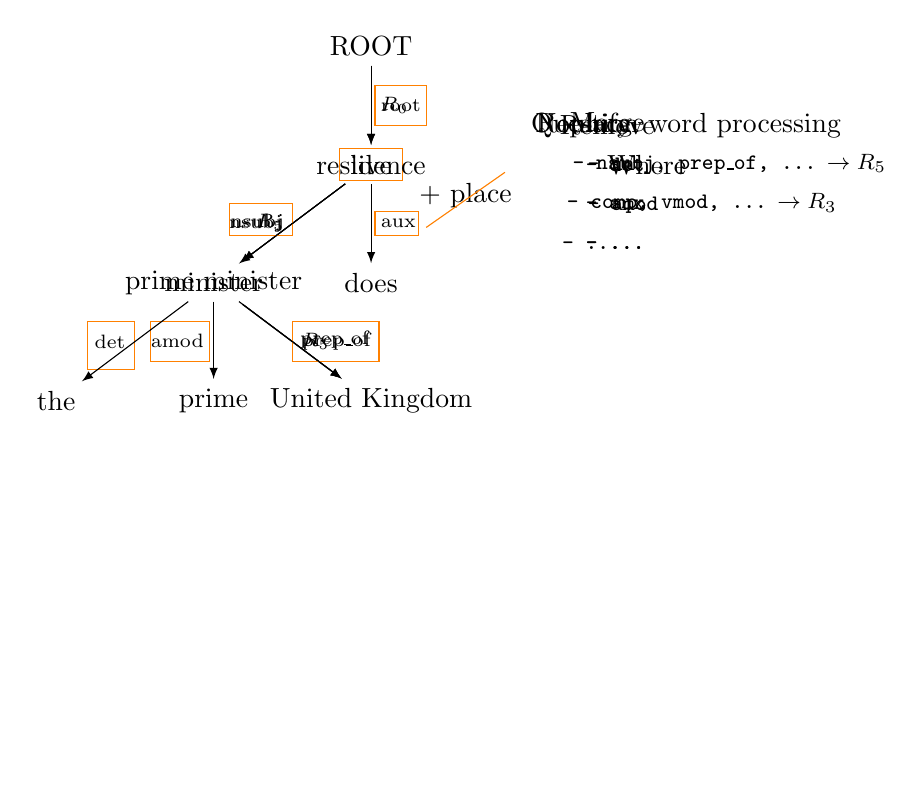
\begin{tikzpicture}
  \node (0) at (10,10) {ROOT};
  \onslide<1-7>{\node (1) at (10,8.5) {live};}
  \onslide<1-3>{\node (2) at (8,7) {minister};}
  \onslide<1>{\node (3) at (10,7) {does};}
  \onslide<1>{\node (5) at (6,5.5) {the};}
  \onslide<1-3>{\node (6) at (8,5.5) {prime};}
  \node (7) at (10,5.5) {United Kingdom};

  \node (8) at (14,1) {}; % utilisé pour forcer le positionnement de la figure globale

  \onslide<1>{\draw [draw=orange] (6.4,6.5) rectangle (7,5.9);}
  \onslide<1>{\draw [draw=orange] (10.05,7.9) rectangle (10.6,7.6);}
  
  \onslide<1,2>{
  \node (9) at (13,9) {\alert{Remove}};
  \node (10) at (13.1,8.5) {\footnotesize{\texttt{- det}}}; 
  \node (11) at (13.1,8) {\footnotesize{\texttt{- aux}}}; 
  \node (12) at (13.1,7.5) {\footnotesize{\texttt{- ...}}};}

  \onslide<3>{\draw [draw=orange] (7.2,6.5) rectangle (7.95,6);}
  
  \onslide<3,4>{
  \node (13) at (13,9) {\alert{Merge}};
  \node (14) at (13.05,8.5) {\footnotesize{\texttt{- nn}}}; 
  \node (15) at (13.2,8) {\footnotesize{\texttt{- amod}}}; 
  \node (16) at (13.1,7.5) {\footnotesize{\texttt{- ...}}};}
  
  \onslide<1-5>{\draw[->, >=latex] (0) edge node[anchor=center, right] {\scriptsize{root}} (1);}
  \onslide<1-3>{\draw[->, >=latex] (1) edge node[anchor=center, left] {\scriptsize{nsubj}} (2);}
  \onslide<1>{\draw[->, >=latex] (1) edge node[anchor=center, right] {\scriptsize{aux}} (3);}
  \onslide<1>{\draw[->, >=latex] (2) edge node[anchor=center, left] {\scriptsize{det}} (5);}
  \onslide<1-3>{\draw[->, >=latex] (2) edge node[anchor=center, right] {\scriptsize{prep\_of}} (7);}
  \onslide<1-3>{\draw[->, >=latex] (2) edge node[anchor=center, left] {\scriptsize{amod}} (6);}

  \onslide<4->{\node (17) at (8,7) {prime minister};}
  \onslide<4-5>{\draw[->, >=latex] (1) edge node[anchor=center, left] {\scriptsize{nsubj}} (17);}
  \onslide<4-5>{\draw[->, >=latex] (17) edge node[anchor=center, right] {\scriptsize{prep\_of}} (7);}

  \onslide<5>{\draw [draw=orange] (10.05,9.5) rectangle (10.7,9);}
  \onslide<5>{\draw [draw=orange] (8.2,8) rectangle (9,7.6);}
  \onslide<5>{\draw [draw=orange] (9,6.5) rectangle (10.1,6);}

  \onslide<5-6>{
  \node (18) at (12.7,9) {\alert{Replace}};
  \node (19) at (14.55,8.5) {\footnotesize{\texttt{- nsubj, prep\_of, ...} $\rightarrow R_5$}}; 
  \node (20) at (14.2,8) {\footnotesize{\texttt{- comp, vmod, ...} $\rightarrow R_3$}}; 
  \node (21) at (12.8,7.5) {\footnotesize{\texttt{- ...}}};}

  \onslide<6->{\draw[->, >=latex] (0) edge node[anchor=center, right] {\scriptsize{$R_0$}} (1);}
  \onslide<6->{\draw[->, >=latex] (1) edge node[anchor=center, left] {\scriptsize{$R_5$}} (17);}
  \onslide<6->{\draw[->, >=latex] (17) edge node[anchor=center, right] {\scriptsize{$R_5$}} (7);}

  \onslide<7-8>{\node (18) at (12.7,9) {\alert{Nounify}};}
  \onslide<7>{\draw [draw=orange] (9.6,8.7) rectangle (10.4,8.3);}
  \onslide<8->{\node (22) at (10,8.5) {residence};}

  \onslide<9-10>{
  \node (23) at (14,9) {\alert{Question word processing}};
  \node (24) at (13.5,8.5) {Where};}

  \onslide<10>{\node (25) at (11.2,8.1) {+ place};
  \draw[orange] (10.7,7.7) -- (11.7,8.4);}
 \end{tikzpicture}
\end{figure}
  
\end{frame}

%#############################################################################################################%
%#############################################################################################################%

\begin{frame}[fragile]
  \frametitle{Local transformations}
  
\begin{figure}
 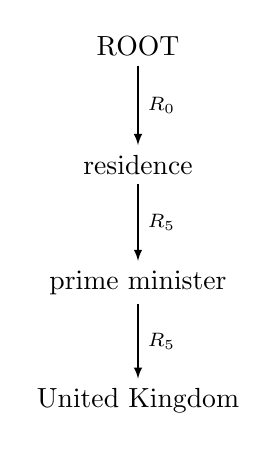
\begin{tikzpicture}
  \node (0) at (10,10) {ROOT};
  \node (1) at (10,8.5) {residence};
  \node (2) at (10,7) {prime minister};
  \node (3) at (10,5.5) {United Kingdom};

  \draw[->, >=latex] (0) edge node[anchor=center, right] {\scriptsize{$R_0$}} (1);
  \draw[->, >=latex] (1) edge node[anchor=center, right] {\scriptsize{$R_5$}} (2);
  \draw[->, >=latex] (2) edge node[anchor=center, right] {\scriptsize{$R_5$}} (3);  
 \end{tikzpicture}
\end{figure}

\end{frame}

%#############################################################################################################%
%#############################################################################################################%

\begin{frame}[fragile]
  \frametitle{Normalization}
  
\begin{figure}
 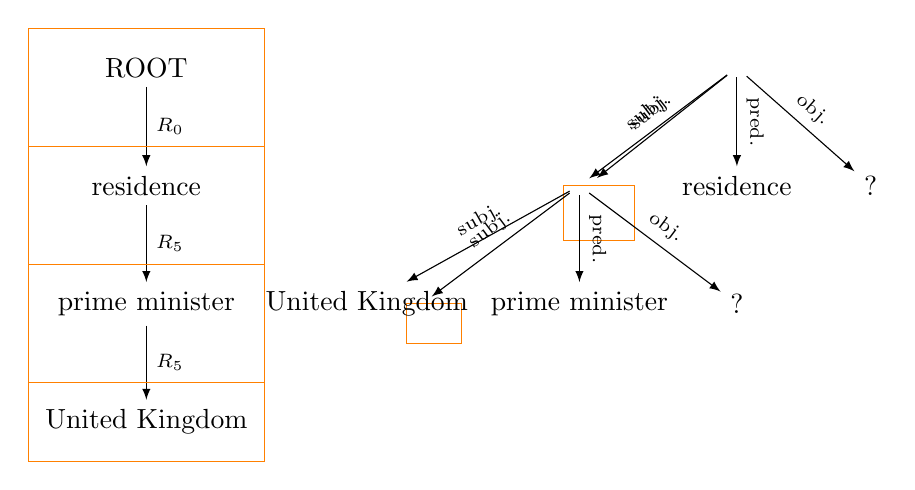
\begin{tikzpicture}
  \node (0) at (9,10) {ROOT};
  \node (1) at (9,8.5) {residence};
  \node (2) at (9,7) {prime minister};
  \node (3) at (9,5.5) {United Kingdom};

  \draw[->, >=latex] (0) edge node[anchor=center, right] {\scriptsize{$R_0$}} (1);
  \draw[->, >=latex] (1) edge node[anchor=center, right] {\scriptsize{$R_5$}} (2);
  \draw[->, >=latex] (2) edge node[anchor=center, right] {\scriptsize{$R_5$}} (3); 
  
  \onslide<1>{\draw [draw=orange] (7.5,10.5) rectangle (10.5,5);}
  \onslide<2>{\draw [draw=orange] (7.5,9) rectangle (10.5,5);}
  \onslide<3>{\draw [draw=orange] (7.5,7.5) rectangle (10.5,5);}
  \onslide<4>{\draw [draw=orange] (7.5,6) rectangle (10.5,5);}

  %%%%
  
  \onslide<3->{
  \node (4) at (16.5,10) {$\triple$};
  \node (5) at (14.6,8.5) {};
  \node (6) at (16.5,8.5) {residence};
  \node (7) at (18.2,8.5) {?};

  \draw[->, >=latex] (4) edge node[sloped, anchor=center, above] {\scriptsize{pred.}} (6);
  \draw[->, >=latex] (4) edge node[sloped, anchor=center, above] {\scriptsize{obj.}} (7); }
  \onslide<3>{\draw[->, >=latex] (4) edge node[sloped, anchor=center, above] {\scriptsize{subj.}} (5);}
  
  \onslide<3>{\draw [draw=orange] (14.3,8.5) rectangle (15.2,7.8);}

  \onslide<4->{
  \node (8) at (14.5,8.5) {$\triple$};
  \node (9) at (12.5,7) {};
  \node (10) at (14.5,7) {prime minister};
  \node (11) at (16.5,7) {?};

  \draw[->, >=latex] (4) edge node[sloped, anchor=center, above] {\scriptsize{subj.}} (8);
  \draw[->, >=latex] (8) edge node[sloped, anchor=center, above] {\scriptsize{pred.}} (10);
  \draw[->, >=latex] (8) edge node[sloped, anchor=center, above] {\scriptsize{obj.}} (11); }

  \onslide<4>{\draw[->, >=latex] (8) edge node[sloped, anchor=center, above] {\scriptsize{subj.}} (9);}

  \onslide<4>{\draw [draw=orange] (12.3,7) rectangle (13,6.5);}
  
  \onslide<5>{\node (12) at (11.8,7) {United Kingdom};
  \draw[->, >=latex] (8) edge node[sloped, anchor=center, above] {\scriptsize{subj.}} (12);}

 \end{tikzpicture}
\end{figure}

\end{frame}

%#############################################################################################################%
%#############################################################################################################%
\iffalse
\begin{frame}[fragile]
  \frametitle{Normalization}
  
\begin{figure}
 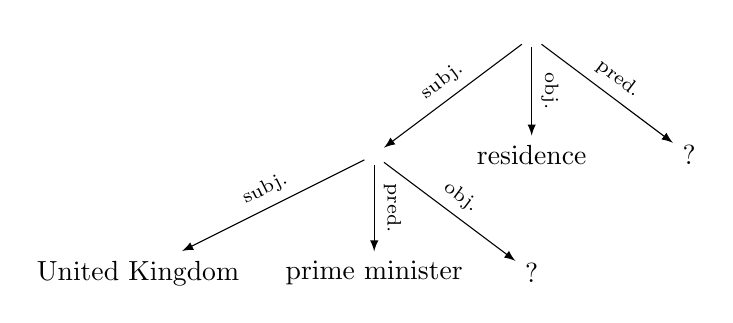
\begin{tikzpicture}
  \node (0) at (10,10) {$\triple$};
  \node (1) at (10,8.5) {residence};
  \node (2) at (12,8.5) {?};
  \node (3) at (8,8.5) {$\triple$};
  \node (4) at (8,7) {prime minister};
  \node (5) at (5,7) {United Kingdom};
  \node (6) at (10,7) {?};

  \draw[->, >=latex] (0) edge node[sloped, anchor=center, above] {\scriptsize{pred.}} (2);
  \draw[->, >=latex] (0) edge node[sloped, anchor=center, above] {\scriptsize{obj.}} (1);
  \draw[->, >=latex] (0) edge node[sloped, anchor=center, above] {\scriptsize{subj.}} (3);
  \draw[->, >=latex] (3) edge node[sloped, anchor=center, above] {\scriptsize{subj.}} (5);
  \draw[->, >=latex] (3) edge node[sloped, anchor=center, above] {\scriptsize{obj.}} (6);
  \draw[->, >=latex] (3) edge node[sloped, anchor=center, above] {\scriptsize{pred.}} (4);
 \end{tikzpicture}
\end{figure}

\end{frame}
\fi
%#############################################################################################################%
%#############################################################################################################%

\begin{frame}[fragile]
  \frametitle{Answer extraction}
  
\begin{figure}
 \begin{tikzpicture}
  \onslide<1-4>{\node (0) at (10,10) {$\triple$};}
  \onslide<1-4>{\node (1) at (10,8.5) {residence};}
  \onslide<1-3>{\node (2) at (12,8.5) {?};}
  \onslide<1-2>{\node (3) at (8,8.5) {$\triple$};}
  \onslide<1-2>{\node (4) at (8,7) {prime minister};}
  \onslide<1-2>{\node (5) at (5,7) {United Kingdom};}
  \onslide<1>{\node (6) at (10,7) {?};}

  \onslide<1-4>{\draw[->, >=latex] (0) edge node[sloped, anchor=center, above] {\scriptsize{pred.}} (1);}
  \onslide<1-3>{\draw[->, >=latex] (0) edge node[sloped, anchor=center, above] {\scriptsize{obj.}} (2);}
  \onslide<1-2>{\draw[->, >=latex] (0) edge node[sloped, anchor=center, above] {\scriptsize{subj.}} (3);}
  \onslide<1-2>{\draw[->, >=latex] (3) edge node[sloped, anchor=center, above] {\scriptsize{subj.}} (5);}
  \onslide<1-2>{\draw[->, >=latex] (3) edge node[sloped, anchor=center, above] {\scriptsize{obj.}} (6);}
  \onslide<1-2>{\draw[->, >=latex] (3) edge node[sloped, anchor=center, above] {\scriptsize{pred.}} (4);}
  
  \onslide<2>{\node (7) at (11,7) {\alert{David Cameron}};}
  \onslide<3-4>{\node (8) at (7.5,8.5) {\alert{David Cameron}};}
  \onslide<4>{\node (9) at (12.5,8.5) {\alert{10 Downing Street}};}

  \onslide<3-4>{\draw[->, >=latex] (0) edge node[sloped, anchor=center, above] {\scriptsize{subj.}} (8);}
  \onslide<4>{\draw[->, >=latex] (0) edge node[sloped, anchor=center, above] {\scriptsize{obj.}} (9);}

  \onslide<5->{\node (10) at (10,10) {\alert{10 Downing Street}};}
  \onslide<5->{\node (11) at (7,7) {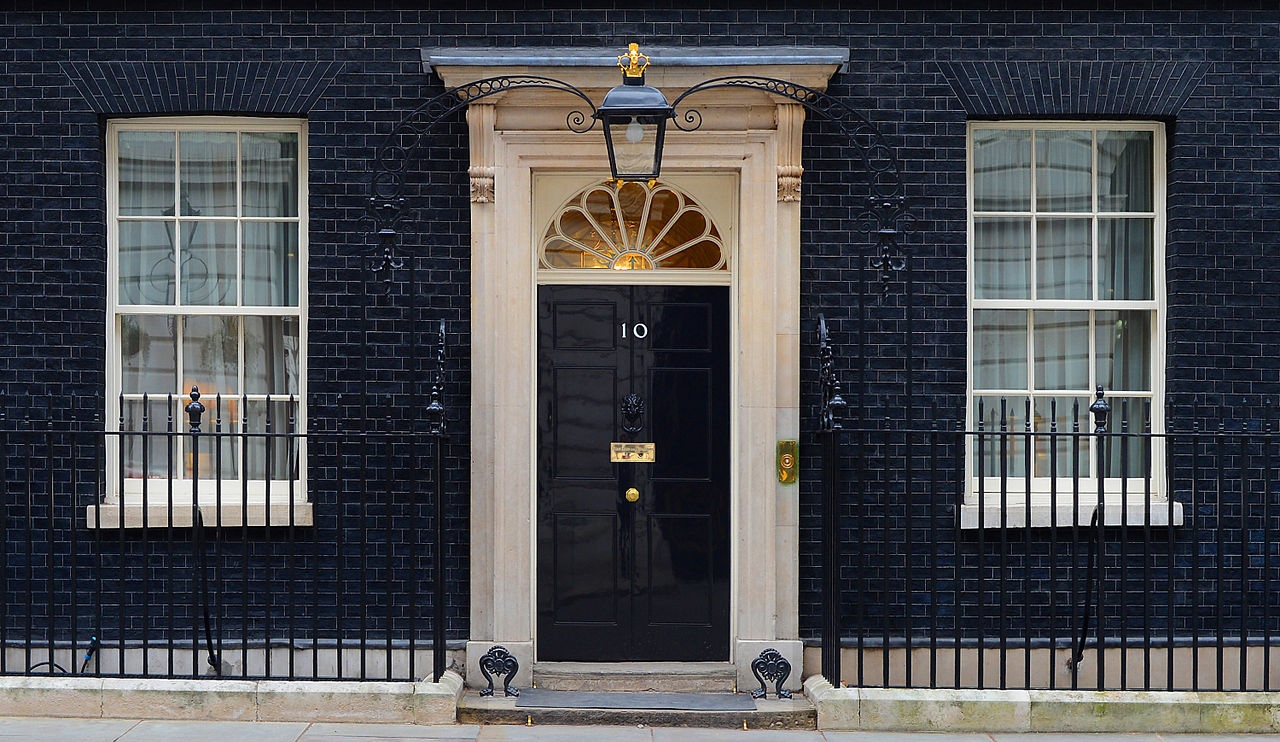
\includegraphics[scale=0.5]{figures/down.jpg}};}
  
  \onslide<2>{\draw[->, >=latex] [draw=orange] [bend right=15, above] (7) edge (3);}
  \onslide<4>{\draw[->, >=latex] [draw=orange] [bend right, above] (9) edge (0);}
 \end{tikzpicture}
\end{figure}

\end{frame}

%#############################################################################################################%
%#############################################################################################################%
